\section{Application Logic - abccore}

This module was created by Matthias Pilot and Nico Wördenweber. In many parts of this module it is not clear to say which one of us is solely responsible for methods of the classes or submodules, as in general we worked closely together. A perfect example for this would be the logic of the Agent class, since it started to be solely Matthias' part, but soon after finishing the first iteration of the data object structure, Nico joined in and provided some of the logic of the Agent, too, where those methods were closer related to the data than to functionality.

\paragraph{Note} that, before going into too much detail, there are some things to be keep in mind throughout this chapter. The main actor in our system is called an agent. The class Agent represents this actor and builds the functions any user has. Although the Agent will be discussed later, note that any user may have multiple instances of the Agent running, and each of these can hold multiple key pairs used to issue transactions in the system. Also, we use Transaction, Acknowledge, Checkpoint, Genesis and Wallet to denote data objects.

A Validator is an Agent whose main purpose is to confirm correct Transaction objects. Whereas a user may be solely interested in spending and receiving money, a Validator earns money by the amount of work it puts into the confirmation of transactions and the creation of checkpoints. However, every running Agent acts automatically as Validator, but the users reward will be much smaller if the Agent only runs while the user actively participates int he system by sending money.

\subsection{Local Data Handling}
\label{local_data_handling}
In this section, Nico explains the parts of the group project he were mainly responsible for, and how they affected the intermediate and final versions of the project.

In the project group ROTRANS, Nicos part was to work mainly with the DAG representation, its corresponding data and handling the local data for the main actor of the project, the Agent. To get a better understanding of what Nicos part in the group was, we start this chapter by visiting the core of our project representation, the DAG. After this, we will provide an abstract overview over the functions maintained by Nico and then go into detail on the checkpoint injection process. The last part of this chapter will be a personal note by Nico on the project and this module.

\paragraph{DAG.py} contains the general structure of the data objects handled in our project and provides small functions related to these objects. In a granular view, the Wallet object is one of the most important parts of the project, as it holds the actual money of the system. For explanation purpose, a Wallet can be seen as a piggy bank with its owners name on it, meaning that it can ever only be opened once to take money out. For functional purpose, the Wallet holds information about one of the public keys of its owner, its own value and state, and is uniquely identifiable.
Any Wallet will be contained in an instance of the class Node, which is the superclass of Transaction, Acknowledge, Genesis and Checkpoint.

A Transaction is the next larger object we need to handle in our project, when it comes to representation. Naturally, a Transaction holds one or multiple Wallets to spent and again one or multiple Wallets which are the result of the transaction. Besides the input and output Wallets, a Transaction also holds information about a delegated Validator, which gains the value of this transaction as stake in the next Checkpoint, and one cryptographical signature for each Wallet in the list of spent Wallets. We speak of a valid Transaction, if and only if for every Wallet in the input list, there is one valid signature signed with the secret key of that Wallets owner.

Closely related to the Transaction, an Acknowledge object represents the vote of a user confirming the correctness of one Transaction. For this, an Acknowledge holds as information the unique identifier of the corresponding Transaction and a signature. An Agent will always created one Acknowledge for each key pair he owns. An Acknowledge also holds the unique identifier of the previous Acknowledge signed with the same key, allowing to track back all Transactions acknowledged by one key.

To provide each Agent instance an initial wallet distribution our cryptocurrency uses an hardcoded genesis, loaded and saved in the Genesis object. It represents the initial wealth and stake distribution in our system and therefore holds Wallets for the initial Agents to use.

Lastly, to enable users to join the system at any time, we introduced Checkpoints to our system. This class was constructed and maintained by our dedicated subgroup. 

\paragraph{In an abstract view,} the file \texttt{agent.py} is the "brain" of our application. The file was mostly developed in close partnership of Matthias, Amin and Nico. One of the first things done in the Agent is recovering its memory, by using the \texttt{load\_data()} function. 

The \texttt{load\_data()} function starts a process to restore a previous session of the user by receiving and parsing data from a SQL database, implemented in \texttt{save\_handler.py}. The user specific data will be saved mostly in the data layer implemented in \texttt{AgentData.py.} The DAG is stored in a dedicated datastructure implemented in \texttt{prefix\_tree.py}

After data from a previous session has been restored and the Agent connected the cryptocurrency system, the user can participate by issuing transactions. The obvious action for this is by using the function \texttt{\_\_send\_money()}, implemented by Matthias. The function uses subroutines on the data layer for assuring the correctness and consistency of the Transactions, namely the functions \texttt{get\_transaction\_set(value)}, \texttt{outputs\_helper()} and \texttt{\_\_create\_signature()}. The Transaction object generated there is then published to the network.

By this point, the Agent is probably already participating as a Validator by receiving Transaction objects from the network and acknowledging valid ones. For this, the function \texttt{\_\_add\_transaction()} checks the consistency and correctness of any incoming Transaction and decides if the Transaction will be declined or added to a list of yet unconfirmed Transactions. Transactions, which are based on yet unconfirmed or unknown Transactions will be added to a list of orphaned Transactions instead.

Any Transaction that is added to the list of unconfirmed Transactions and which is considered valid, will then be acknowledge by the Agent, using the function \texttt{\_\_acknowledge()}. This function leverages the function \texttt{acknowledge()} of the \texttt{AgentData} to create or retrieve Acknowledge objects corresponding to the Transaction. These Acknowledges are then sent over the network.

Similar to receiving Transactions from the network, the Agent can receive Acknowledge objects. These are handled in the \texttt{\_\_add\_acknowledgement()}. After validation of the signatures in the Acknowledge object, the function checks if the corresponding Transaction is in the list of unconfirmed Transactions. In that case, the Acknowledge is counted for that Transactions needed stake. If a Transaction gains enough stake like this to be considered confirmed, the function \texttt{\_\_add\_confirmed\_trans()} removes the Transaction from the list of unconfirmed Transactions and adds it to the DAG representation in memory and the local database.

An Agent continually tries to guarantee consistent data by sending requests to the network. The function \texttt{\_\_retry\_missing\_txn\_request()} is used to regularly ask for Transactions missing to process unconfirmed Transactions and unprocessed Nodes.

Another major part of the Agent is to handle Checkpoints. The checkpoint service calls the function \texttt{inject\_checkpoint()} of the Agent for this. This function then starts the transition process by calling the function \texttt{switch\_to\_ckpt()}, which itself initates the transformation of the DAG to the new checkpoint state. While the data layer transforms the DAG, the latter function reevaluates Nodes which were already processed but not part of the Checkpoint and sends requests for unknown Transactions which were mentioned in the Checkpoint. After \texttt{switch\_to\_ckpt()} is done, the function \texttt{inject\_checkpoint()} recalculates the stake threshold new Transactions need to reach to be confirmed, based on the new checkpoint. 

Lastly, the Agent will regularly save the session data using the function \texttt{save\_data()}, leveraging the function of same name of the data layer. Similar to the \texttt{load\_data()}, the data will be parsed and then saved in a SQL database.

\paragraph{Checkpoint injection} is one of the most complex tasks of the Agent. Besides reevaluating Nodes which weren't included in the Checkpoint, there are a lot of other tasks to be done to ensure a consistent transition. To emphasize this, we will describe the routines needed for this transition in more detail, starting with a view behind the curtain of the data layer. Code~\hyperref[pseudo_transform_dag_1]{3.1} shows one half of an abstract pseudo code of the function \texttt{transform\_dag()} of the class \texttt{AgentData}.

\begin{center}
\label{pseudo_transform_dag_1} \small \samepage
\begin{verbatim}
TRANSFORM_DAG:   
  Delete current save of this session

  Create a new tree and add all previous checkpoints

  Add unspent TXNs to the tree
  For all unspent transaction outputs in the checkpoint:
     Add Wallet to utxo_set search for its dependend nodes

     Check if TXN of this Wallet is in tree or put it in set 
     missing_txn_requests
     
     Set this Wallet to UNSPENT

     Set the TXNs parents to this ckpt

  Add TXN.identifier to set of kept TXNs and add the TXN to 
  the new tree

  Add Checkpoint to new tree
...
\end{verbatim}	
\vspace{2mm}	
\footnotesize{Code~\hyperref[pseudo_transform_dag_1]{3.1}: First part of the pseudo code of function \texttt{transform\_dag()}.}
\end{center}

The first part here is to delete the currently used database. This is not the backup created by the function \texttt{switch\_to\_cpkt()}, but the database which is saved to and load from per default.
In this part of the functions pseudo code, the Transactions of the old tree will be copied to the new tree, only if they are marked as (partially) unspent by the Checkpoint. By keeping the original Transactions, we can ensure that no adversarial party in the checkpoint committee can manipulate the unspent Transactions, since all Transactions are signed once for each PK of one of its input Wallets. Also, for these Transactions, the attribut parents will be set to the Checkpoints unique identifier, establishing a line of trust from this checkpoint on, because the past of this Transaction will probably not be available after the transition.
The second part of this pseudo code describes that unspent Wallets will be used to search for their dependend nodes. This will be a part in the second half of the pseudo code. Also, All Wallets mentioned in the Checkpoint will be set to \texttt{UNSPENT}, ensuring that reevaluation of confirmed but not in the Checkpoint included Transactions will succeed.

\begin{center}
\label{pseudo_transform_dag_2} \small \samepage \centering
\begin{verbatim}
...
  For all unspent transaction outputs:
     If output belongs to one of this Agents keys, add it 
     to its balance

  For all rewards in the Checkpoint:
     If reward belongs to one of this Agents keys, add it 
     to its balance

  Search for TXNs which were confirmed while the ckpt was 
  created and mark them as deconfirmed

  For all deconfirmed Nodes in the old tree
     Add the TXNs to set pending_trans and reset them to UNSPENT

     Add the ACKs to set pending_acks

  For all TXNs in the old pending_transactions
     Add received ACKs to pending_acks

     Add TXNs to pending_trans

     Add all acks for this TXNs outputs and inputs to 
     mapping retained_wallets

  Override local acked_wallets with retained_wallets

  Override local tree with new_tree

  For each key of this Agent, set the last_ack to the 
  new Checkpoint

  Return pending_trans, pending_acks, missing_txn_requests
\end{verbatim}
\vspace{2mm}	
\footnotesize{Code~\hyperref[pseudo_transform_dag_2]{3.2}: Second part of the pseudo code of function \texttt{transform\_dag()}.}
\end{center}

Code~\hyperref[pseudo_transform_dag_2]{3.2} shows the second half of the pseudo code of the function  \\\texttt{transform\_dag()} of the class \texttt{AgentData}. In the first part of Code~\hyperref[pseudo_transform_dag_2]{3.2}, the balance of the Agent will be recomputed over the unspent transaction outputs and the rewards listed in the Checkpoint. This ensures, that the users balance is kept consistent with the Transactions confirmed directly after the transition. Note that this means, that if the user had spent Wallets contained in the Checkpoint prior to its injection, those Wallets will now be added back to the Agents balance. This is necessary to enable the correct reevaluation of the made Transactions and does not threaten the correctness of the system as detailed below. 
As already mentioned, the Transactions which were confirmed while the Checkpoint was created will be labeled deconfirmed and added to a set of \texttt{pending\_txns}, with their Wallets set to \texttt{UNSPENT}. Also, all Transactions which were pending before will also be added to that set for reevaluation. To ensure correctness and to consistency of the system, all Acknowledges of Transactions in the set \texttt{pending\_txns} are added to a set of \texttt{pending\_acks}. This will also be reevaluated, directly after this function finishes, to ensure that the user can not spent Wallets twice by accident. Also in this part of the pseudo code, it is mentioned that the mapping \texttt{retained\_wallets} will override the mapping \texttt{acked\_wallets}. The latter one maps a Wallet to a list of Acknowledges, and holds mappings for all Wallets of Transactions, which the Agent had acknowledged. This is a list, because for each Transaction, the Agent will create one Acknowledge for each of its key pairs. \texttt{retained\_wallets} holds only mappings of those Wallets which can still be accessed after the transition, meaning all inputs and outputs of Transactions in the new tree or in the \texttt{pending\_txns}.
Then, to ensure correctness and a line of trust in the future Acknowledges of this Agent, the attribute \texttt{last\_ack} will be set to this Checkpoints identifier for each key pair of this Agent.
Lastly, the sets \texttt{pending\_trans}, \texttt{pending\_acks} and \texttt{missing\_txn\_requests} will be returned.

\begin{figure}[htbp]
	\centering
	\label{fig:code_switch}
	\includegraphics[width=0.9\textwidth, trim={0cm 0cm 0cm 0cm},clip]{figures/nico/code_switch}
	
	\footnotesize{Figure~\hyperref[fig:code_switch]{3.3}: Python code of function \texttt{switch\_to\_cpkt()}.}
\end{figure}

Now, with the function \texttt{transform\_dag()} described above, Figure~\hyperref[fig:code_switch]{3.3} shows the actual Python code of the function \texttt{switch\_to\_cpkt()} of the Agent. 
This function first creates a backup of the session, before starting the transaformation on the data layer by calling the function \texttt{transform\_dag()} to receive the sets \texttt{pending\_trans}, \texttt{pending\_acks} and \texttt{missing\_txn\_requests}. After the transformation of the tree is done, the function calls a helper function to remove unprocessed Nodes, from the corresponding list named \texttt{orphaned\_nodes}, which were already in that list before the previous checkpoint was processed.
The next step is to clear the list of pending transactions, since all of those Transactions were added to the set \texttt{pending\_trans} in the function \texttt{transform\_dag()}. This ensures, that those Transactions will be evaluated in the next step, as if they were just received over the network. To quickly reconfirm Transactions that were deconfirmed in the transition process, the Acknowledges in the set \texttt{pending\_acks} will also be evaluated as if they were just received. To finish the process, this function requests the Transactions for all identifiers in the set \texttt{missing\_txn\_requests} and saves the session data in a new database.































\subsection{Network, UI and Checkpoint Interface}
The Agent module is the heart of the the whole logic and data structure. It brings all gearwheels together and therefore, needs a special architecture as depicted in Figure~\hyperref[interface_overview]{3.4}.
For a more detailed overview over the dependencies of the abccore module see Figure~\hyperref[agent_dependencies]{3.5}
The Agent extends the class AgentMessageHandler which is responsible for handling messages from the Network.
This inheritance allows the Agent itself to actually handle messages from the network.
Sending own messages back to the network can be done over a special ChannelService which is given within the constructor of the AgentMessageHandler.

For the UI establishing the Agent also extends the LocalMessageHandler class. This class offers the UI multiple predefined method calls such as \texttt{send\_money} and the direct access to the Agent memory.
Updates can only be initialized on the UI side, the Agent itself has no opportunity to initialize a communication to the UI.

For the injection of new computed checkpoints the checkpoint service can call the method \texttt{inject\_checkpoint(ckpt)} which will overwrite the current state of the DAG.
Besides this the checkpoint service also has access to the Agents memory to be able to negotiate new checkpoints. 

\begin{figure}[h]
	\centering
	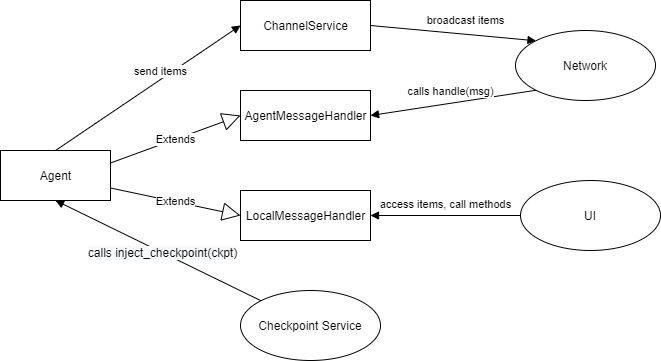
\includegraphics[scale=0.7,trim={1cm 18.5cm 0cm 0cm}, origin=c, clip ]{figures/drawio/class_diagram_overview.pdf}
    \footnotesize{Figure~\hyperref[interface_overview]{3.4}:~Interface~Overview~from~an~Agents~Side}
    \label{interface_overview}
\end{figure}

\begin{figure}[h]
	\centering
	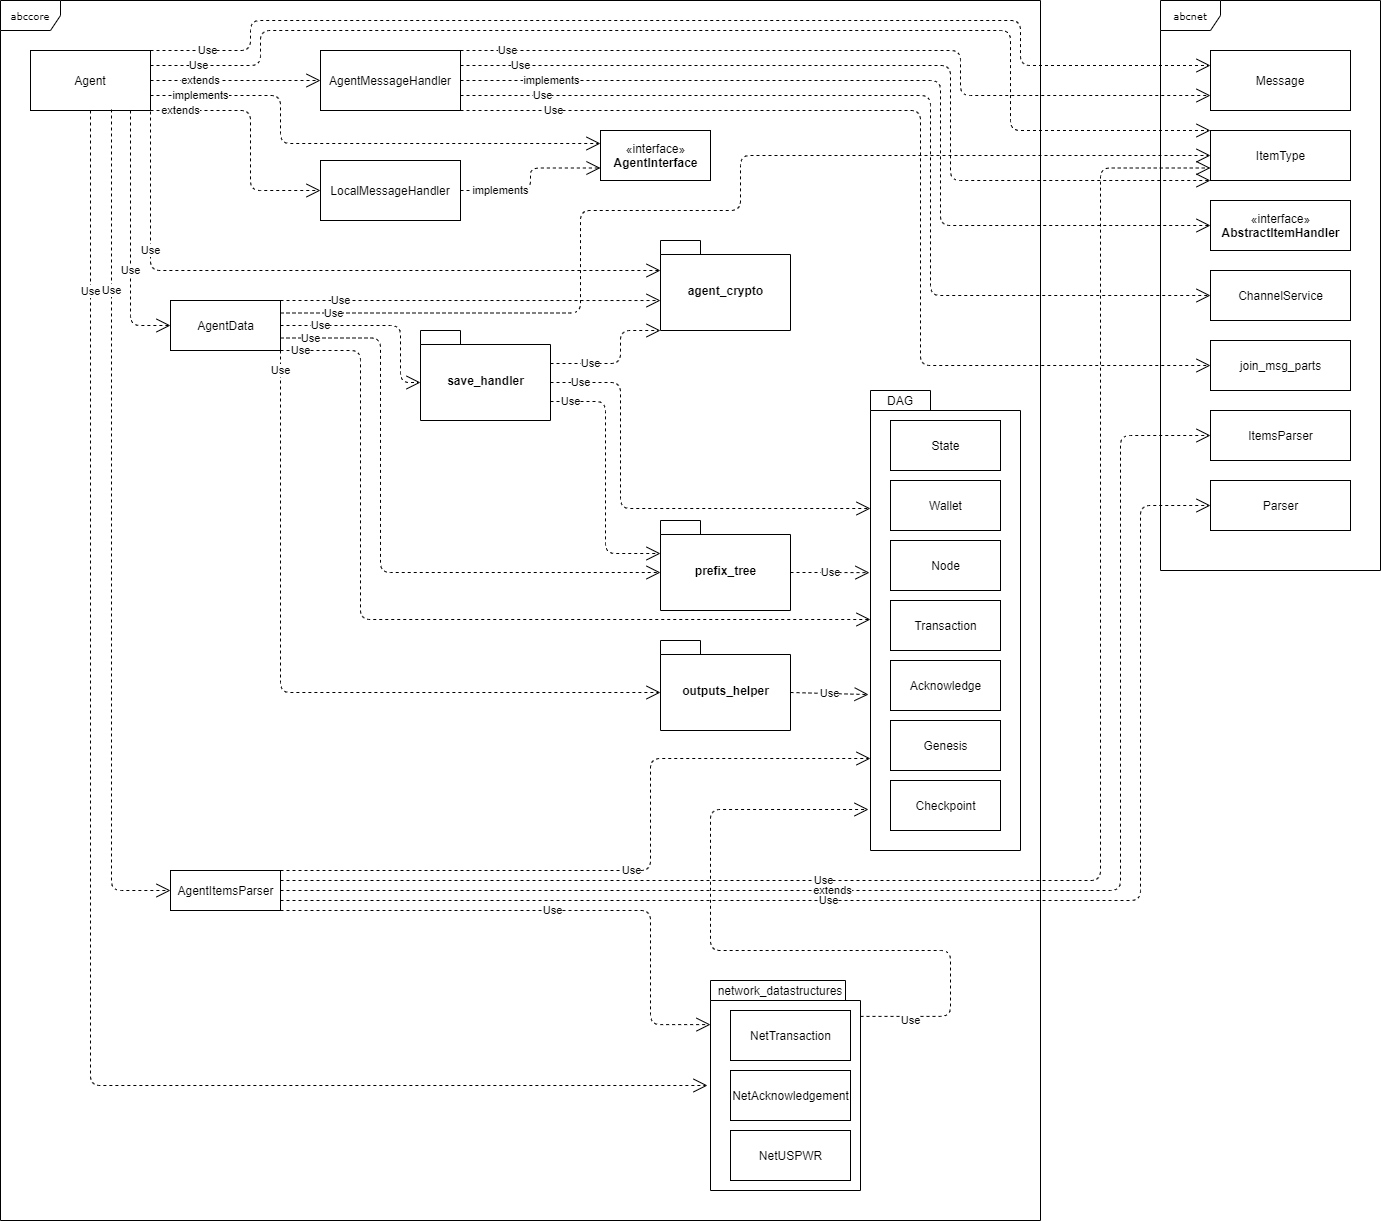
\includegraphics[scale=0.45, trim={0cm 0cm 0cm 0cm},clip]{figures/drawio/agent_dependencies.pdf}
	\footnotesize{Figure~\hyperref[interface_overview]{3.5}:~Agent~Dependency~Diagram}
	\label{agent_dependencies}
\end{figure}


\subsection{Data Preparation for the Network-Agent Interface}
\label{data_prep}
Our implementation of the ABC-protocol is build for a distributed environment. Since all communication and messages are generally broadcasted to the whole network sending each new acknowledgement, transaction or unspent-wallet-request message one by one can harm the throughput of the whole network.
Further, directly reacting to new messages from the network can lead to much more traffic. The Push-and-Pull protocol we are using for the network first provides checklists of IDs for the network so remote agents can request these new items on demand.
If an agent receives a new checklist of new item-IDs it might request the network for the actual content by sending a fetch-item list which includes the IDs of the requested items as well.
Eventually, if an remote agent has the underlying content to the corresponding ID this remote agent will send the content within a item list.
If we now imagine a system where each remote agent directly reacts to new messages the whole network would be overflowed with checklists, fetch-item lists and item-lists each consisting of single elements. Additionally, messages can be received in a different order they were send due to possible delays on the network layer, so further additional requests for items which are already sent to the network are created.

\begin{figure}[h]
	\centering
	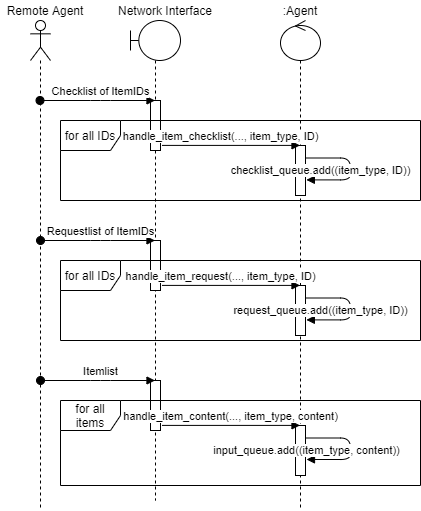
\includegraphics[scale=0.8,trim={0cm 15cm 10cm 0cm}, origin=c, clip ]{figures/drawio/sequence3.pdf}
    \footnotesize{Figure~\hyperref[input_queues]{3.6}:~Checklist,~Requestlist~and~Itemlist~Handling}
    \label{input_queues}
\end{figure}

To prevent this overflowing with messages the Agent class first collects all incoming messages in the \texttt{input\_queue} for all items of received item lists, in the \texttt{request\_queue} for all item IDs of received fetch-item lists and in the \texttt{checklist\_queue} for all item IDs of received checklists as pictured in Figure~\hyperref[input_queues]{3.6}.


For the \texttt{checklist\_queue} and the \texttt{request\_queue} we use \texttt{set()} as datatype, so duplicates e.g. received due to different checklists of different agents are directly eliminated.
Since we also want to prevent spamming attacks by the agent itself created by fast item-generation like transactions we use this system not only for incoming items but for outgoing items as well.
The Agent first collects all created items like transactions or acknowledgements and prepares the outgoing checklist, fetch-item list and item-list.
After a certain amount of time the BaseApp will call the method \texttt{perform\_maintenance()} of the Agent which basically works through all the incoming items to make method calls for further proceeding and all the outgoing lists to propose new items and item requests to the network.



To actually  send items to the network as already mentioned in Section~\ref{local_data_handling}  the Agent first has to prepare and transform them.
For this purpose the Agent makes use of the datatypes NetTransaction, NetAcknowledgement and NetUSPWR (= Net-Unspent-Wallet-Request).
These are necessary because the for the internal data structure used objects do not include necessary properties to be encodeable and decodeable for the network purpose in a useful manner.
Only these three "Net"-item types can be send from an Agent instance.


\subsection{Replay Function}
During the runtime of our distributed system new agents may join or will go offline to join again to a later point in time.
Since new agents only know the genesis and previously offline agents only know the latest status before they turned offline we had to implement a replay functionality to our system.
First, after start-up the checkpoint service will get the latest checkpoint from the network and inject it into our Agent instance.
Now the Agent instance has to replay all transactions since this checkpoint or, if this state is actually newer, from his last state on.
To do so the Agent instance collects all unspent wallets and sends them to the network with help of the specific NetUSPWR datatype as described in Section~\ref{data_prep}.
If a remote Agent instance will receive such a request it will resend all transactions and acknowledgements which have been sent after the by the NetUSPWR specified unspent-wallets.
The previously offline Agent can now just add all objects he does not know to his local AgentData structure.


\subsection{Example Run Throughs}

\subsubsection{Example: Sending Money}
In the following we will show an example run through of the \\
\texttt{send\_money(value,recipient,validator)} method which is also shown in \\Figure~\hyperref[send_money]{3.7}.
This method is called if a new transaction is initialized within the UI.
The call will then be forwarded to the AgentData class.
Since wallets are handled like piggy banks and can only be used as whole we can not just take the needed money of one wallet.
Instead, we are processing our owned wallets and set up a wallet set which is able to pay the needed value and the additional fee which will be needed for submitting the transaction.
This is done by the method \texttt{get\_transaction\_set(value)}.
Further, the resulting wallets will most probably not match the exact value we need for the transaction and the additional fee.
Therefore, we use the method \texttt{outputs\_helper} to actually compute the wallets we want to spend to the transaction's recipient and one wallet which will set up a new wallet for the Agent itself to store the rest of the input wallets money which has not been used.
After the input and output wallets have been successfully computed the Agent can now setup the transaction itself.
To proof the ownership of the input wallets the Agent now signs the transaction with all secret keys which belong to the owner public keys of the input wallets.
The transaction can only be validated successfully later if the transaction is signed by each owner key of these input wallets.
After the transaction is initialized the Agent itself will create a NetTransaction object to propose the new transaction to the network.
This new NetTransaction item is now added to the outgoing checklist queue as described in Section~\ref{data_prep}.
Now, the Agent will acknowledge the transaction with all of his keypairs and therefore, its whole amount of stake.
Since transactions are only confirmed if at least $\frac{2}{3}$ of the stake in the whole network acknowledged it, it is important to actually acknowledge this new transaction with as much own stake as possible.
Each created Acknowledge object will have exactly one signature, namely the signature of the keypair this acknowledgements public key hints to.
After the AgentData class has acknowledged the new transaction with all of its keys it will return a list of the newly created acknowledgements to the Agent instance.
The process of acknowledging new transactions we just ran through even is the same for new transactions received by the network. Of course validation is a very important part here as well (even if the transaction is created by ourself) but this would go too much into deep.
Now, similar as for the transaction object, the Agent will create several NetAcknowledgement objects to prepare the Acknowledge objects for sending over the network.
Again, the newly created NetAcknowledgement objects are added to our outgoing checklist so they can be actually send within the next \texttt{perform\_maintenance()} call.
Since transaction creation, validation and acknowledgement creation is now complete the \texttt{send\_money(...)} call is finished.
By sending the transaction and the own acknowledgements within the same checklist in the \textbf{next} \texttt{perform\_maintenance()} call we can again reduce the number of single messages in the network.


\begin{figure}[h]
	\centering
	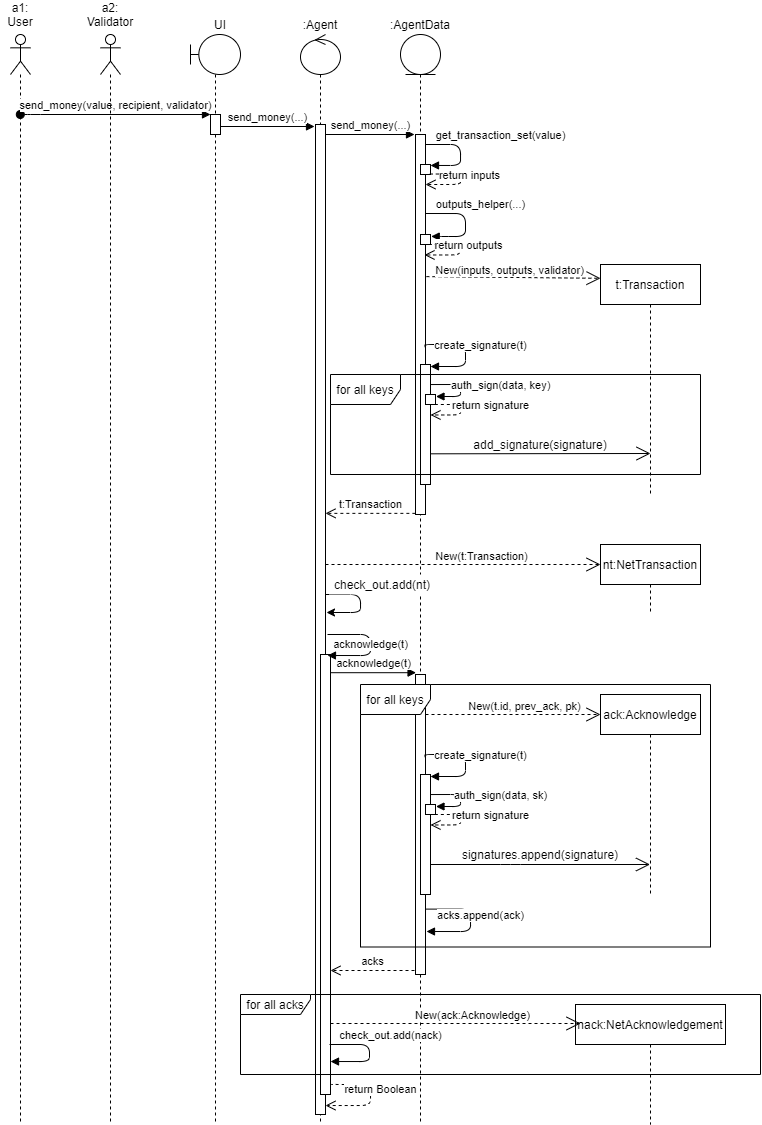
\includegraphics[width=0.8\textwidth, trim={0cm 0cm 0cm 0cm},clip]{figures/drawio/sequence1.pdf}
	\footnotesize{Figure~\hyperref[send_money]{3.7}:~"Send~Money"~Run~Through}
    \label{send_money}
\end{figure}

\subsubsection{Example: Generating/Adding new Keypairs}
The following run through is shown in Figure~\hyperref[sequence2]{3.8}.
If the user wants to generate a new keypair he can click the button "Generate Keys" in the UI.
The UI will forward the call to the corresponding Agent instance which further forwards it to AgentData and the "cryptography" module \cite{pypi_crypt} related methods in the "agent\_crypto.py".
After generation the key will be added to the keyset by the AgentData instance of the Agent.
After the key has been added the UI will call an update from the Agent to actually show the newly created keypair in the UI.

If the user wants to add a new keypair manually, e.g. because he wants to synchronize his wallets over multiple devices, he can just press the "+" button in the UI and enter the secret key he wants to add in hexadecimal representation.
The UI will forward the call to agent, which will further forward it to the AgentData instance to actually add the newly created secret key to the database.
For the keygeneration and signatures we use elliptic curve Diffie-Hellmann Ed25519 of the open source "cryptography" library \cite{pypi_crypt}.
Since this public key encryption scheme allows to compute the public keys out of the private key submitting only the private key is sufficient to add the whole keypair to the keyset of AgentData.


\begin{figure}[h]
	\centering
	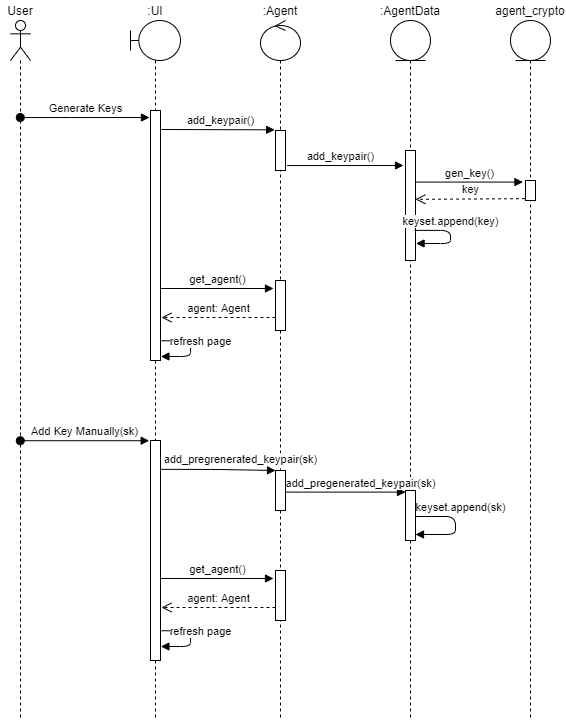
\includegraphics[width=0.8\textwidth, trim={0cm 0cm 0cm 0cm},clip]{figures/drawio/sequence2.pdf}
	\footnotesize{Figure~\hyperref[sequence2]{3.8}:~"New~Keypair"~Run~Through}
	\label{sequence2}
\end{figure}

